\documentclass{article}
\usepackage{amsmath}
\usepackage{amssymb}
\usepackage{amsthm}
\usepackage{verbatim}
\usepackage{graphicx}
\usepackage{enumerate}
%\usepackage{figure}


%\usepackage{caption}
%\usepackage{subfig}
%\usepackage{enumitem}

%\usepackage{caption}
%\usepackage{epstopdf}
%\usepackage{float}


\theoremstyle{plain}
  \newtheorem{theorem}{Theorem}[section]
  \newtheorem{prop}[theorem]{Proposition}
  \newtheorem{cor}[theorem]{Corollary}
  \newtheorem{lemma}[theorem]{Lemma}
  \newtheorem{claim}[theorem]{Claim}
\theoremstyle{definition}
  \newtheorem{defn}[theorem]{Definition}
  \newtheorem{exmp}[theorem]{Example}
  \newtheorem{obs}[theorem]{Observation}
  \newtheorem{remark}[theorem]{Remark}
  \newtheorem{construction}[theorem]{Construction}


\title{Exploring Bounds}
\author{Tyler Friedman}


\begin{document}
\maketitle

\section{Introduction}

\begin{comment}
PLAN
do elias, don't prove first lemma, prove second lemma and thm
do given examples, draw graphs
finish out examples of lexicodes
add graphs to plotkin
finish analysis of asymptotic singleton and plotkin
\end{comment}

An interesting problem in coding theory is determining the maximum
number of codewords in a code with certain parameters.  For an $n$-dimensional code, we are interested in 
the maximum number of codewords such that the code has minimum distance $d$.  
Formally, we use the notation $A_q(n,d)$
and $B_q(n,d)$ to define the maximum of number of codewords in a code over
$\mathbb{F}_q$ of length $n$ and minimum distance $d$ for an arbitrary (linear
on non-linear) code and linear code, respectively.  

For arbitrary $n$ and $d$, it is difficult to find $A_q(n,d)$ and $B_q(n,d)$ exactly.
 In lecture, we have considered upper bounds---Sphere Packing, Singleton, and Greismer---as well as
lower bounds---Gilbert and Varshamov---on these values.  The purpose of this
paper is to take a survey of other well-known bounds in the literature that we have not discussed.  
In the first part of the paper, we will consider the Plotkin Upper bound, 
the Elias Upper bound.  In the second part of the paper, we will consider the asymptotic versions of the Singleton, Plotkin, and Elias bounds.  Lastly, in the final part we will consider lexicodes, an interesting subset of linear codes that meet the Gilbert Bound.

\section{Upper Bounds}

\subsection{Plotkin Upper Bound}

The Plotkin Bound is an upper bound that often improves upon the Sphere Packing Bound on $A_q(n,d)$.

\begin{theorem}[Plotkin]
Let $C$ be an $(n,M,d)$ code over $\mathbb{F}_q$ such that $rn < d$ where $r = 1 - q^{-1}$.  Then
\begin{equation}
A_q(n,d) \le \left \lfloor \frac{d}{d-rn}\right\rfloor
\end{equation}
\end{theorem}

Before proving this bound, it is important to note that it is only valid when $d$ is sufficiently close to $n$.  For large $q$, this is can be a considerable limiting factor.
Consider that our restriction is $n<2d$ for $q=2$, $n<\frac{3}{2}d$ for $q=3$, $n<\frac{4}{3}d$ for for $q=4$, etc.


\begin{proof}
Let 
\begin{equation} \label{plotkin_1}
S = \sum_{x \in \mathcal{C}} \sum_{y \in \mathcal{C}} \text{d}(x,y)
\end{equation}

Note that for $x,y \in \mathcal{C}$, d$(x,y)=0$ for $x=y$, and $d \le$ d$(x,y)$ for $x\neq y$.  This implies that
\begin{equation} \label{plotkin_1_5}
M(M-1)d\le S
\end{equation}

This comes directly from equation \ref{plotkin_1}.  We have $M$ possible codewords to consider for $x$ in the outer summation, $M-1$ distinct codewords from $x$ to consider in the inner summation for $y$, 
and the distance between $x$ and $y$ will always be greater than or equal to the minimum distance $d$.

Next, let $\mathcal{M}$ be the $M \times n$ matrix whose rows are the codewords of $\mathcal{C}$.  For $1 \le i \le n$, let $n_{i,\alpha}$ be the number of times $\alpha \in
 \mathbb{F}_q$ occurs in column $i$ of $\mathcal{M}$.  Note that $\sum_{\alpha \in \mathbb{F}_q} n_{i,\alpha} = M$ for $1\le i \le n$.  This is simply because there are $M$ total
 elements of $\mathbb{F}_q$ in each column, so the sum over all $n_{i,\alpha}$ must necessarily be $M$.  

I claim that we can rewrite $S$ as a double sum over these $n_{i,\alpha}$ values.  Specifically,

\begin{equation}
S = \sum_{i=1}^{n} \sum_{\alpha\in\mathbb{F}_q} n_{i,\alpha}(M - n_{i,\alpha}).
\end{equation}

Note that $n_{i,\alpha}(M - n_{i,\alpha})$ is multiplying the number of times $\alpha$ occurs in column $i$ by the number of times it doesn't occur in column $i$.  In other words, we're counting the number of times two elements of the same
column are not equivalent, exactly the condition that constitutes the Hamming distance.   By summing over all $\alpha$ and then all columns, we arrive at the same value generated by \ref{plotkin_1}.

Next, simplify:

\begin{equation}
\begin{split}
\sum_{i=1}^{n} \sum_{\alpha\in\mathbb{F}_q} n_{i,\alpha}(M - n_{i,\alpha}) &= M\sum_{i=1}^{n} \sum_{\alpha\in\mathbb{F}_q} n_{i,\alpha} - \sum_{i=1}^{n} \sum_{\alpha\in\mathbb{F}_q} n_{i,\alpha}^2 \\
&= nM^2 - \sum_{i=1}^{n} \sum_{\alpha\in\mathbb{F}_q} n_{i,\alpha}^2
\end{split}
\end{equation}

Recall the Cauchy-Schwarz inequality, which states that $\left(\sum_{i=1}^n x_i y_i \right )^2 \le \left(\sum_{i=1}^n x_i^2 \right ) \left(\sum_{i=1}^n y_i^2 \right )$
For our purposes, this means that $\left(\sum_{\alpha\in\mathbb{F}_q} 1\cdot n_{i,\alpha} \right )^2 \le q \left(\sum_{\alpha\in\mathbb{F}_q} n_{i,\alpha}^2 \right )$.

Using this inequality, we obtain

\begin{equation} \label{plotkin_2}
S \le nM^2 - \sum_{i=1}^n q^{-1} \left(\sum_{\alpha\in\mathbb{F}_q} 1\cdot n_{i,\alpha} \right )^2 = nM^2 - \frac{nM^2}{q} = nrM^2.
\end{equation}

Combining \ref{plotkin_1_5} and \ref{plotkin_2}, we get $M(M-1)d \le nrM^2$, which simplifies to 

\begin{equation}
M \le \left\lfloor \frac{d}{d-rn} \right\rfloor.
\end{equation}

\end{proof}

It is interesting to see exactly how the Sphere Packing and Plotkin bounds compare for specific values of $n$ and $d$.  For the following examples we will assume $q=2$.    
Also, recall that if $d$ is even, $A_2(n,d) = A_2(n-1,d-1)$.  

\begin{exmp}
$(n,d) = (7,4)$.

Applying the Sphere Packing bound, we have $A_2(7,4) = A_2(6,3) \le \frac{2^6}{1 + 6}$, 
giving us $A_2(7,4) \le \textbf{9}$.

Applying the Plotkin bound, we have $A_2(7,4) \le \frac{4}{4-\frac{1}{2}\cdot7} = \textbf{8}$.

\end{exmp}

\begin{exmp}
$(n,d) = (9,6)$.

Applying Sphere Packing, we have  $A_2(9,6) = A_2(8,5) \le \frac{2^8}{1+8+28}$, giving us $A_2(n,d) \le \textbf{6}$.

Applying the Plotkin bound, we have $A_2(9,6) \le \frac{6}{6-\frac{1}{2}\cdot9} = \textbf{4}$.
\end{exmp}

Using MATLAB, I sought to visualize how the Plotkin and Sphere Packing bounds compare.  To do so, I plotted their values over $8\le n \le 25$, with $d>rn$.  Below is the case
of $q=2$; I found similar but more smoothed out results for higher values of $q$ (see submission folder).

\begin{figure}[ht]
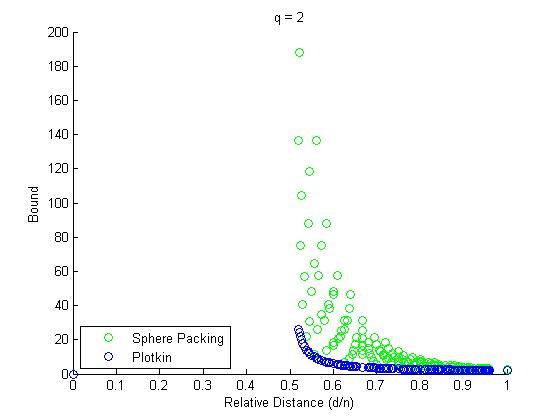
\includegraphics[width=.8\linewidth]{plotkin_q2.png}
\caption{Plotkin and Sphere Packing bounds for $n,d\in[8,25]$}
\end{figure}
I also thought it would be interesting to visualize how the Plotkin bound and Sphere Packing bounds operate as a function of $n$ and $d$.  Given various values of $n$ and $d$, I plotted the resulting bound, 
and then used Delaunay triangulation [REFERENCE] to turn the discrete 3D data into a smooth mesh surface.  (See Sphere Packing data on next page).  

\begin{figure}
\centering
\begin{minipage}[b]{0.45\linewidth}
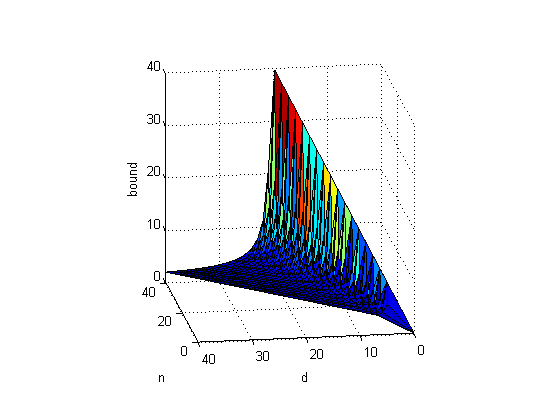
\includegraphics[width=1.4\linewidth]{plotkin.png}
\label{fig:minipage1}
\end{minipage}
\quad
\begin{minipage}[b]{0.45\linewidth}
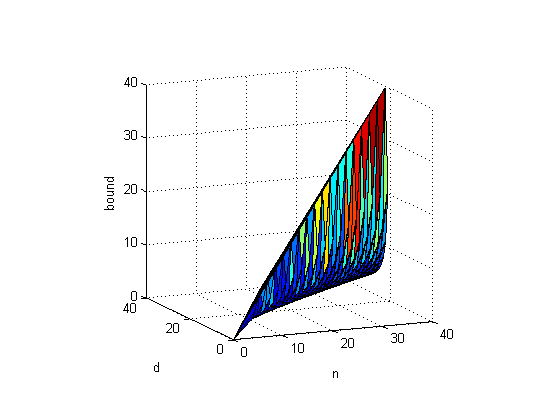
\includegraphics[width=1.4\linewidth]{plotkin_2.png}
\label{fig:minipage2}
\end{minipage}
\caption{Two different perspectives of the same graph, the Plotkin Bound for $q$=2, $n,d\in[6,40]$ }
\end{figure}

\begin{figure}
\centering
\begin{minipage}[ht]{0.45\linewidth}
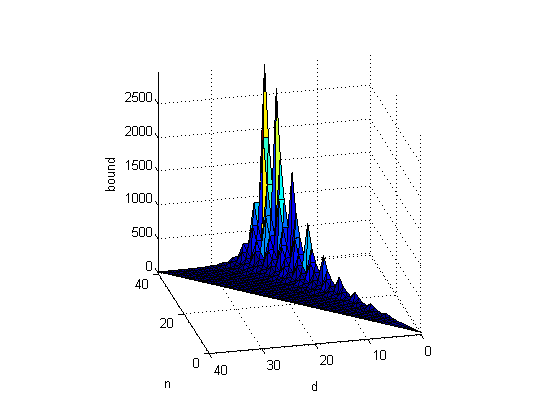
\includegraphics[width=1.4\linewidth]{sp_1.png}
\label{fig:minipage1}
\end{minipage}
\quad
\begin{minipage}[ht]{0.45\linewidth}
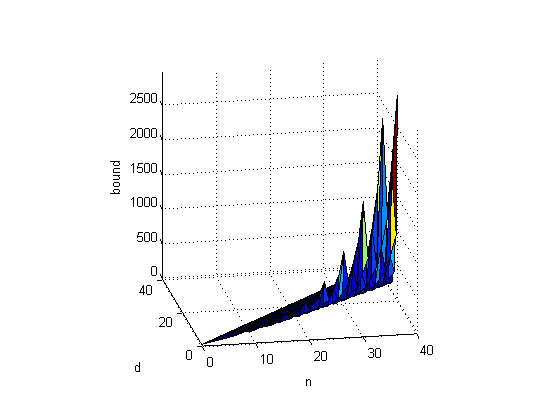
\includegraphics[width=1.4\linewidth]{sp_2.png}
\label{fig:minipage2}
\end{minipage}
\caption{Two different perspectives of the same graph, the Sphere Packing Bound for $q$=2, $n,d\in[6,40]$ }
\end{figure}


\subsection{Elias Upper Bound}

Another upper bound on $A_q(n,d)$ is due to Elias in 1960.  The Elias bound is generally weaker than other bounds we have discussed, but is important because of the asymptotic
form that it generates.

In order to prove the Elias bound, two lemmas are necessary.

\begin{lemma}
Let $\mathcal{C}$ be an $(n,K,d)$ code over $\mathbb{F}_q$ such that all codewaords have weights at most w, where $w \le rn$ with $r=1-q^{-1}$.  Then
\begin{equation}
d\le \frac{Kw}{K-1}\left(2- \frac{w}{rn}\right).
\end{equation}
\end{lemma}

The proof of this lemma uses a very similar technique to that used in our proof of the Plotkin bound. Just as before, given an $(n,K,d)$ code $\mathcal{C}$, the proof considers
the $K \times n$ matrix $\mathcal{M}$ whose rows are the codewords of $\mathcal{C}$.  Using this matrix, the proof takes the expression $K(K-1)d$ and shows through a number of equation manipulations
that it is less than or equal the expression $K^2 w\left( 2 - \frac{w}{rn}\right )$.  Two key tools for the proof are the Cauchy-Schwartz inequality, and the relationship between 
the sum of the distances between all pairwise codewords and the sums of the $n_{i,\alpha}$ values in the columns of $\mathcal{M}$.

As an aside: the second lemma, stated below, uses the notation $V_q(n,a)$ to denote the number of vectors in a sphere of radius $a$ in $\mathbb{F}_q^n$.  This is a concept 
that we became very familiar with this semester in our discussions of the Sphere Packing and Gilbert bounds.

\begin{lemma}
Suppose C is an (n,M,d) code over $\mathbb{F}_q$.  Then there is an $(n,M,d)$ code $\mathcal{C}'$ over $\mathbb{F}_q$ with an (n,K,d) subcode $\mathcal{A}$ containing
only codewords of weight at most w such that $K \ge M V_q(n,w) / q^n$.
\end{lemma}

The proof of this lemma begins by considering the intersection between a sphere of radius w centered at $\mathbf{0}$, and the special vector $x\in \mathbb{F}_q^n$ added to $\mathcal{C}$ such that the intersection
is maximal.  The important step is noticing that this value is greater than or equal to the sum over all vectors $y\in\mathbb{F}_q^n$ of that same sphere of radius $w$, intersected with 
$y+\mathcal{C}$, all divided by $q^n$.  The proof then uses sum manipulations to find a relationship between our original expression and $\frac{1}{q^n}V_q(n,w)M$.

\begin{theorem}
Let $r=  1-q^{-1}$.  Suppose that $w\le rn$ and $w^2 - 2rnw + rnd > 0$.  Then

\begin{equation}
A_q(n,d) \le \frac{rnd}{w^2 - 2rnw + rnd}\cdot \frac{q^n}{V_q(n,w)}.
\end{equation}
\end{theorem}

The proof of this theorem, though omitted, follows almost directly from the previous two lemmas.

We can work through a few examples to see how the Elias bound operates.

\begin{exmp}
$n=14$, $d=6$, $q=2$. 
Recall from before that $A_2(n,d)=A_2(n-1,d-1)$ if $d$ is even.  We will again use this fact to find the best possible bound that this theorem can provide. 

 For $w=0$, 
we get $A_2(13,5)\le \frac{.5\cdot13\cdot5}{.5\cdot13\cdot5}\cdot\frac{2^{13}}{V_q(13,0)} = 2^{13} = 8192$; similarly, $A_2(14,6) = 2^{14} = 16384$.

 For $w=1$, 
we get $A_2(13,5)\le \frac{.5\cdot13\cdot5}{1 - 2\cdot.5\cdot13 + .5\cdot13\cdot5}\cdot\frac{2^{13}}{V_q(13,1)} = \frac{32.5}{1-13+32.5}\cdot\frac{2^{13}}{1+13} = 927$;
similarly $A_2(14,6)\le \frac{.5\cdot14\cdot6}{1 - 2\cdot.5\cdot14 + .5\cdot14\cdot6}\cdot\frac{2^{14}}{V_q(14,1)} = \frac{42}{1-14+42}\cdot\frac{2^{14}}{1+14} = 1581$.

For $w=2$, 
we get  $A_2(13,5)\le \frac{.5\cdot13\cdot5}{4 - 2\cdot2\cdot.5\cdot13 + .5\cdot13\cdot5}\cdot\frac{2^{13}}{V_q(13,2)} = \frac{32.5}{4-26+32.5}\cdot\frac{2^{13}}{1+13+78} = 275$;
similarly $A_2(14,6)\le \frac{.5\cdot14\cdot6}{4 - 2\cdot2\cdot.5\cdot14 + .5\cdot14\cdot6}\cdot\frac{2^{14}}{V_q(14,2)} = \frac{42}{4-28+42}\cdot\frac{2^{14}}{1+14+91} = 360$.

For $w=3$, 
we get  $A_2(13,5)\le \frac{.5\cdot13\cdot5}{9 - 2\cdot3\cdot.5\cdot13 + .5\cdot13\cdot5}\cdot\frac{2^{13}}{V_q(13,3)} = \frac{32.5}{9-39+32.5}\cdot\frac{2^{13}}{1+13+78+286} = 281$;
similarly $A_2(14,6)\le \frac{.5\cdot14\cdot6}{9 - 2\cdot3\cdot.5\cdot14 + .5\cdot14\cdot6}\cdot\frac{2^{14}}{V_q(14,3)} = \frac{42}{9-42+42}\cdot\frac{2^{14}}{1+14+91+ 364} = 162$.

For $w=4$,
in the case of $A_2(13,5)$, the first denominator is less than zero, and thus we cannot apply the bound; $A_2(14,6)$ still works, however.  
$A_2(14,6)\le \frac{.5\cdot14\cdot6}{16 - 2\cdot4\cdot.5\cdot14 + .5\cdot14\cdot6}\cdot\frac{2^{14}}{V_q(14,4)} = \frac{42}{16-56+42}\cdot\frac{2^{14}}{1+14+91+ 364+1001} = 233$.

Thus the best upper bound from the Elias Bound for $A_2(13,5)=A_2(14,6)=162$.

\end{exmp}







\section{Asymptotic Bounds}
We now wish to consider these $A_q(n,d)$ values as n goes to infinity.  To do so, we must more formally define two terms.

In class, we have considered the \textit{rate} of a linear code, $k/n$, as one measure of the goodness of a code.  That is,
the rate tells us how much information relative to redundancy that our codewords provide.  The concept of rate can be generalized
to non-linear codes as well.  For a possibly nonlinear code over $\mathbb{F}_q$ with $M$ codewords, the \textit{rate} is defined to be $n^{-1} \log_q {M}$.  Notice that
for an $[n,k,d]$ linear code, $M = q^k$ and hence the rate is $k/n$ as we expect.

A second notion of goodness that we have discussed, but I think not formally defined, is the \textit{relative distance} of a code.  For a linear or nonlinear code of length n
has minimum distance d, this value is the ratio $d/n$. 

For our asymptotic bounds, we are interested in the largest
possible rate for a family of codes over $\mathbb{F}_q$ of lengths going to
infinity with a relative distance of some constant $\delta$.  In other words, we consider the equation:

\begin{equation}
\alpha_{q}(\delta) = \limsup_{n \to \infty} n^{-1} \log_q A_q(n,\delta n)
\end{equation}

To better understand what is going on here, consider the case of an $[n,k,d]$ linear code $\mathcal{C}$.  Before, we wanted to know how large we could get $k$ given
$n$ and $d$.  Now, we want to know how large we can get $\frac{k}{n}$ given $\frac{d}{n}=\delta$ as $n\to\infty$.  This idea generalizes to non-linear codes as 
in the non-asymptotic cases we discussed in class.

For the rest of this section, we will consider two bounds on $A_q(n,\delta n)$

\subsection{Asymptotic Singleton Bound}

Recall the Singleton Bound from lecture:

\begin{theorem}
For $d \le n$, $A_q(n,d) \le q^{n-d+1}$.
\end{theorem}

The asymptotic bound follows almost directly from the non-asymptotic variation.

\begin{theorem}
If $0 \le \delta \le 1$, then $\alpha_q(\delta) \le 1 - \delta$.
\end{theorem} 


\begin{proof}
\begin{equation} 
\begin{split}
\alpha_{q}(\delta) & = \limsup_{n \to \infty} n^{-1} \log_q A_q(n,\delta n) \\
& \le \limsup_{n \to \infty} n^{-1} \log_q q^{n-\delta n+1} \\
& \le \limsup_{n \to \infty} \frac{n-\delta n+1}{n} \\
& \le 1 - \delta
\end{split}
\end{equation}
\end{proof}

\subsection{Asymptotic Plotkin Bound}
The Asymptotic Plotkin Bound gives a small improvement on the Asymptotic Single Bound.  

\begin{theorem}
Let $r=1-q$.  Then 
\begin{equation*}
\alpha_q(\delta)= 
\begin{cases} 0, &\mbox r\le\delta\le1 \\ 1-\delta/r, &\mbox{} 0\le\delta < r. \end{cases}
\end{equation*}
\end{theorem}

\begin{proof}[Sketch of proof]
First, consider the case of $r\le\delta\le1$.  Notice that we can apply the Plotkin bound directly, as $rn < \delta n = d$.  By the Plotkin Bound, $A_q(n,\delta n) \le \frac{\delta n}{\delta n - rn}$.  Cancelling
out the common $n$, we get $A_q(n,\delta n) \le \frac{\delta}{\delta - r}$.  Since this value is independent of $n$, it immediately follows from the definition that $\alpha_q(\delta)=0$.

Next, consider the case of $0\le\delta < r$.  Suppose that $\mathcal{C}$ is an $(n,M,\delta n)$ code where $M=A_q(n,\delta n)$ .  Our goal is to puncture $\mathcal{C}$ such that 
we get a shorter length code $\mathcal{C}'$ with the same minimum distance as $\mathcal{C}$.  The idea is to find a code whose $n$ is small enough that we can still apply the Plotkin bound, and then bound
our original code $\mathcal{C}$ with the shortened code's Plotkin value.
Use a shortening technique analgous to the one we described in lecture, as well as Section 1.5.3 of the textbook,
let $\mathcal{C}'$ be the $(n',M',\delta n)$ code where $n' = \lfloor (\delta n -1)/ r \rfloor$ and $M' \ge M/q^{n-n'}$.  Given this code, we can show that $A_q(n,\delta n) \le q^{n-n'} \delta n$.
Simplifying using the definition of $\alpha_q(\delta)$ completes the proof.
\end{proof}

Once again, we use MATLAB to visually compare two bounds.  This time, we consider the Asymptotic Singleton and Asymptotic Plotkin bounds.  

\begin{figure}[ht]
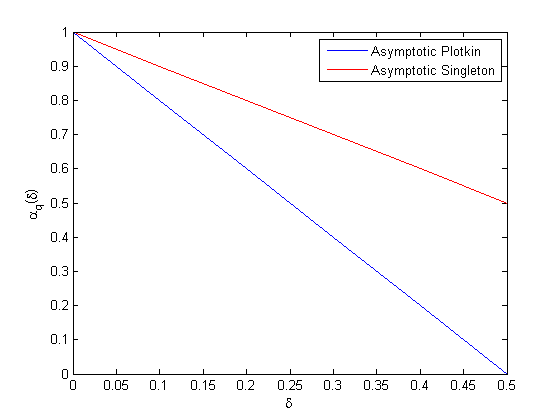
\includegraphics[width=.8\linewidth]{asympt.png}
\caption{Asymptotic Plotkin and Singleton bounds for $q=2$}
\end{figure}

\section{Lexicodes}

We end our discussion on bounds with an interesting class of linear codes
called lexicodes, short for lexicographic codes.  Lexicodes are linear and meet the Gilbert bound; we will discuss the former and prove the latter.  Note that for this discussion we are 
solely working in $\mathbb{F}_2$.

We construct the lexicode $\mathcal{L}(n,d)$ of length $n$ and minimum distance $d$ using a basic greedy algorithm as follows.  First, order all $n$-tuples in an array $A$ in lexicographic order:
$A[0] = 0\cdots000$, $A[1]=0\cdots001$, $A[2]0\cdots010$, $A[3]=0\cdots011$, \ldots, $A[2^n-1] = 1\cdots111$.  Put the first vector from  $A$ (always the $\mathbf{0}$ vector) in $\mathcal{L}$.  Next, find the first vector $\mathbf{x}$
of weight $d$ in the lexicographic ordering, and put it in $\mathcal{L}$.  Then, find the next vector in the lexicographic ordering in $A$ whose distance from each vector in $\mathcal{L}$ is 
$d$ or more and add it to $\mathcal{L}$.  Repeat this process until you have scanned through all of $A$ once.

The set $\mathcal{L}$ is a linear code of length $n$ and minimum distance $d$.  The set $\mathcal{L}$ also contains linear subcodes which are generated by the above algorithm,
but stopping at the right spots.

\begin{theorem}
After constructing $\mathcal{L}$ as above, label the vectors $\mathbf{c}_0$, $\mathbf{c}_1,$ $\ldots$ in the order they were selected such that $\mathbf{c}_0$ is the $\mathbf{0}$ 
vector.

\begin{enumerate}[{\normalfont (i)}]
\item $\mathcal{L}$ is a linear code and the vectors $\mathbf{c}_{2^i}$ are a basis of $\mathcal{L}$.  
\item After $\mathbf{c}_{2^i}$ is chosen, the next $2^i -1$ vectors can be rewritten as $\mathbf{c}_1 + \mathbf{c}_{2^i}$, $\mathbf{c}_2 + \mathbf{c}_{2^i}$, $\ldots$, 
$\mathbf{c}_{2^i -1} + \mathbf{c}_{2^i}$.
\item Let $\mathcal{L}_i = \{\mathbf{c}_0,\mathbf{c}_1,\ldots,\mathbf{c}_{2^i -1}\}$.  Then $\mathcal{L}_i$ is an $[n,i,d]$ linear code.

\end{enumerate}

\end{theorem}

I claim that (i) and (iii) follow from (ii).  For (ii), we are showing that all codewords in the lexicode are simply linear combinations of 
the $c_{2^i}$ codewords, hence making the $c_{2^i}$ codewords a basis for the code.  The sketch of the proof for (ii) involves inducting on $i$.  Essentially, the proof works
by assuming that the second $2^{i}$ vectors in $\mathcal{L}_{i+1}$ are not necessarily generated by adding $\mathbf{c}_2^{i}$ to each of the previously chosen vectors
in $\mathcal{L}_i$.  If you break this assumption, then you can use the notion of lexicographic order to find two vectors lexicographically ordered in a way that is not actually
possible.

The codes $\mathcal{L}_i$ satisfy the inclusions $\mathcal{L}_1 \subset \mathcal{L}_2 \subset \cdots \subset \mathcal{L}_k = \mathcal{L}$, where $k$ is the dimension of 
$\mathcal{L}$.  In general, this dimension value $k$ is not known until you have completed the construction as described above.

We now consider a basic example of a lexicode $\mathcal{L}(n,d)$ and it's $\mathcal{L}_{i}$s.

\begin{exmp}
Consider the codes $\mathcal{L}_i$ of length $5$ and minimum distance $2$.  First, we must construct the entire lexicode $\mathcal{L}$.  To do so, we enumerate
all 32 vectors of $\mathbb{F}_2^5$ in lexicographic order: $00000$,$00001$,$00010$,$\ldots$,$11111$.  We find that $\mathcal{L} = \{00000, 00011,00101,00110,01001,
01010,01100,01111,10001,10010,\\ 10100,10111,11000,11011,11101,11110\}$.  As a sanity check, note that $\left | \mathcal{L} \right | = 16$, a power of $q$.  Consequently, we have
$\mathcal{L}_1 = \{00000,00011\}$, $\mathcal{L}_2 = \{00000, 00011,00101,\\ 00110\}$, $\mathcal{L}_3 = \{00000, 00011,00101,00110,01001,01010,01100,01111\}$, and
$\mathcal{L}_4 = \mathcal{L}$. We can check to make sure that each $\mathbf{c}_j$ is a linear combination of the $\mathbf{c}_{2^i}$s. For this example, consider $\mathcal{L}_3$:

\begin{enumerate}%[start=0]
\item $\mathbf{c}_0$ is the trivial linear combination.
\item $\mathbf{c}_1 = \mathbf{c}_1$
\item $\mathbf{c}_2 = \mathbf{c}_2$
\item $\mathbf{c}_3 = \mathbf{c}_1 + \mathbf{c}_2$.  $00110 = 00011+ 00101$.
\item $\mathbf{c}_4 = 1\cdot\mathbf{c}_4$
\item $\mathbf{c}_5 = \mathbf{c}_1 + \mathbf{c}_4$. $01010 = 00011 + 01001$.
\item $\mathbf{c}_6 = \mathbf{c}_2 + \mathbf{c}_4$. $011000 = 00101 + 01001$.
\item $\mathbf{c}_7 = \mathbf{c}_3 + \mathbf{c}_4 = \mathbf{c}_1 + \mathbf{c}_2 + \mathbf{c}_4$. $01111 = 00011 + 00101+01001$.
\end{enumerate}

The same analysis applies for all $\mathcal{L}_i$s.

\end{exmp}

Note that the greedy algorithm we descibed in the beginning of the section requires a strictly lexigraphical ordering, or else the code that is produced will not necessarily
be linear.  Again consider the case of $\mathbb{F}_2^5$, but instead of the lexigraphical ordering, shift every vector up one such that the ordering is identical to before, except now the
zero vector is at the bottom of the list.  If we run our algorithm on this ordering, we will clearly not choose the zero vector to be a part of $\mathcal{L}$ and hence 
$\mathcal{L}$ will not be linear.  

Also, note that lexicodes meet one of the bound we discussed in lecture, the Gilbert bound.  Recall the Gilbert bound:

\begin{equation}
B_q(n,d) \ge \frac{q^n}{\sum_{i=0}^{d-1} \binom{n}{i}(q-1)^{i}}
\end{equation}

\begin{claim}
Lexicodes meet the Gilbert bound.
\end{claim}

\begin{proof}
Consider an arbitrary lexicode $\mathcal{L}$.  Recall our construction of $\mathcal{L}$ with vectors in $\mathbb{F}_q^n$, wherein we visit each vector in our ordering,
and if it is distance $d$ or more to every current element in $\mathcal{L}$ then we add it to our set.  At the same time, notice that when a vector is visited in our algorithm, 
if it has distance $d-1$ or less to any vector in $\mathcal{L}$, then it is not placed in $\mathcal{L}$.  Since all vectors in $\mathbb{F}_q^n$ are visited in our algorithm, any
$v \in \mathbb{F}_q^n$ must either be in $\mathcal{L}$ or must have distance $d-1$ or less to some vector in $\mathcal{L}$.  Hence the covering radius of $\mathcal{L}$ is $d-1$.  

Consequently, it is enough to show that any code $\mathcal{C}$ with covering radius $d-1$ or less meets the Gilbert bound.  Recall that the Gilbert bound can be thought of as a restatement of the 
following fact: (number of spheres) $\cdot$ (number of vectors in a sphere with radius $d-1$) $\ge$ (number of vectors in $\mathbb{F}_q^n$).  Since our covering radius
is $d-1$ or less, and we have that all codewords are distance $d$ or more apart, consequently no sphere of radius $d-1$ in $\mathbb{F}_q^n$ can contain more than one codeword.
Our spheres will still overlap, however, meaning (number of vectors in
$\mathbb{F}_q^n$)/(number of vectors in a sphere with radius $d-1$) will
certainly be greater than or equal to the number of spheres around codewords.
Hence, $\mathcal{C}$ meets the Gilbert bound.
\end{proof} 

It may be surprising to discover that many codes we have already discussed in lecture are in fact lexicodes.  In order to have this discussion, though, we
first need two important definitions.

\begin{defn}
The $\mathbf{nim-sum}$ NS($v$) of a vector $v \in \mathbb{F}_2^n$ is the sum of
it's coordinates in GF($2$).
\end{defn}

\begin{defn}
A vector $v\in \mathbb{F}_2^n$ is $\mathbf{zero-sum}$ if NS($v$)=0.
\end{defn}

We have used the idea of nim-sums and zero-sums throughout the course, but instead we have
used the terms even-like or odd-like.  In the binary case, these are equivalent notions.

We also need the following Lemma:

\begin{lemma}
The codewords of the lexicode $\mathcal{L}(n,d)$ are also in the lexicode $\mathcal{L}(n+1,d)$, except with an additional leading zero.
\end{lemma}

\begin{proof}
This follows directly from how our algorithm above was constructed.  We obviously have $\mathbb{F}_q^n \subset \mathbb{F}_q^{n+1}$, and in our algorithm these will be
the first $2^n$ vectors that are visited.  Since all that has changed is we've added a leading $0$, the algorithm will choose these same vectors $\mathcal{L}(n,d)$ vectors.
\end{proof}

In lecture, we have frequently discussed the code of all even-weight codewords.  In $\mathbb{F}_2$, this is a lexicode.

\begin{claim}
For $d=q=2$, $\forall v\in \mathcal{L}$, NS($v$) $= 0$, and hence $\mathcal{L}$ is an even-like code.
\end{claim}

\begin{proof}
We will prove this by inducting on $n$.  In the base case of $n=1$,
$\mathcal{L}=\{0\}$, which is trivially zero-sum.  

Assume that, for the lexicode of length $n$, all codewords are zero-sum.  Now, we must show that all
the codewords in $\mathcal{L}(n+1,2)$ are zero-sum as well.  By our lemma, all codewords in $\mathcal{L}(n,2)$ are also in $\mathcal{L}(n+1,2)$, except with an
extra leading zero.  By our assumption, these codewords are still zero-sum, as adding a zero in front will not change the nim-sum calculation.

Let ${\mathbb{F}_q^n}^*$ be the vectors of $\mathbb{F}_q^n$ with a zero appended in front of the first coordinate.  Now, we must show that for the remaining vectors $v\in\mathbb{F}_q^{n+1} \setminus {\mathbb{F}_q^{n}}^*$that we have not yet visited, our algorithm will choose all
even-weight vectors and none of the odd-weight vectors.  

First, consider the odd-weight vectors of $\mathbb{F}_q^{n+1} \setminus {\mathbb{F}_q^{n}}^*$.  Note that 
these are actually just the even weight vectors of $\mathbb{F}_q^n$ with a $1$ appended to the front.  If you flip the first bit of each vector, you get an even weight codeword that
we have already shown to be in $\mathcal{L}(n+1,2)$, and consequently no such odd-weight codeword can be in $\mathbb{L}(n+1,2)$.

Finally, consider the even-weight vectors of $\mathbb{F}_q^{n+1} \setminus {\mathbb{F}_q^{n}}^*$.  Notice that these are just the odd-weight vectors of $\mathbb{F}_q^n$ with a $1$
appended to the front.  By our assumption, none of the odd-weight vectors of ${\mathbb{F}_q^n}^*$ are in $\mathcal{L}(n+1,2)$.  This means that each even-weight
vector in $\mathbb{F}_q^{n+1} \setminus {\mathbb{F}_q^{n}}^*$ will necessarily have distance $2$ from vectors in $\mathcal{L}(n,2)$ (with a zero appended to the front).  We also
have that any two distinct even-weight vectors are at least distance $2$ from one another, as an even-weight vector can only possibly have distance one from an odd-weight vector.  
Hence, all even-weight vectors of $\mathbb{F}_q^{n+1} \setminus {\mathbb{F}_q^{n}}^*$ will be chosen by our algorithm.
\end{proof}

We have also frequently discussed the Hamming codes.  In (insert reference to Greedy Codes paper), they show that the binary lexicodes with $d$=3 and $n=2^m-1$ are the Hamming codes, 
and similarly, as one might expect considering the previous statement, the binary lexicodes with $d=4$ and $n=2^m$ are the extended Hamming codes.  We can check
this with a simple example.

\begin{exmp}
Let $n=7$, $d=3$.  It can be quite tedious to compute and confirm something like this by hand, so I wrote a short C++ program that implements the Lexicode algorithm as described above.  We find $\mathcal{L}(7,3)$ to be $\{0,7,25,30,42,45,51,52,75,76,82,85,97,102,120,127\}$ where the binary vectors are given by their decimal representation.
\end{exmp}

Note that $\mathcal{L}(7,3)$ has $16$ codewords, making it a $[7,4,3]$ code.  Recall that in lecture we proved that all $[7,4,3]$ codes are the Hamming(7,4) code.  

\end{document}
